\documentclass[handout]{beamer}
\usetheme{Boadilla}
\usepackage{graphicx}
\title[Precautionary Savings with Risky Assets]{Precautionary Savings with Risky Assets: \\ When Cash Is Not Cash}
\subtitle{Ran Duchin, Thomas Gilbert, Jarrad Harford, and Chris Hrdlicka \\ Journal of Finance (2017)}
\author{Alex von Hafften}
\institute{UW-Madison}

\begin{document}

\begin{frame}
\titlepage
\end{frame}






\begin{frame}
\frametitle{Motivation}
\begin{itemize}[<+->]
\item Traditional assumption in corporate finance models:

\bigskip

\textit{Financial portfolios of industrial firms are only cash (or near-cash).}

\bigskip

\item But recent media coverage indicates that firms invest in a broader set of financial assets.
\end{itemize}
\end{frame}

\begin{frame}
\frametitle{What do Duchin et al do?}
\begin{itemize}[<+->]
\item Measure the financial portfolios of large U.S. industrial firms.
\bigskip
\item Show how risky financial asset holdings change with firm characteristics.
\end{itemize}
\end{frame}

\begin{frame}
\frametitle{Key Findings}
\begin{itemize}[<+->]
\item U.S. industrial firms invest heavily in risky financial assets
\begin{itemize}[<+->]
\item 40\% of aggregate financial asset portfolio
\item 6\% of aggregate book value
\end{itemize}
\bigskip
\item Investments in risky financial assets are higher for less financially constrained firms.
\end{itemize}
\end{frame}

\AtBeginSubsection[ ]
{
\begin{frame}{Outline}
    \tableofcontents[currentsubsection]
\end{frame}
}

\section{Summary of Duchin et al (2017)}

\subsection{Measurement}



\begin{frame}[label=standardapproach]
\frametitle{Standard Approach to Measure Financial Portfolios}
From consolidated balance sheet,
\bigskip
\begin{itemize}[<+->]
\item ``Cash and cash equivalents" ($CH$ in Compustat)
\begin{itemize}
\item Financial assets with maturity of up to 90 days at issuance.
\end{itemize}
\bigskip
\item ``Short-term investments" ($IVST$)
\begin{itemize}
\item Financial assets that the firm intends to liquidate within a year.
\end{itemize}

\bigskip
\item The standard measure of financial assets is $CHE = CH + IVST$

\bigskip

\item \textbf{Problem: Underestimate because $CHE$ omits financial assets in ``long-term investments" and ``other assets".}
\end{itemize}
\bigskip


\hyperlink{APPL2007}{\beamerskipbutton{Apple 2007 10-K}}

\end{frame}


\begin{frame}[label=duchinapproach]
\frametitle{Duchin et al (2017) Approach}
\begin{itemize}[<+->]
\item In 2009, the SEC began requiring firms to disclose more information about their financial assets. \hyperlink{APPL2011}{\beamerskipbutton{Apple 2011 10-K}}
\bigskip
\item Duchin et al. (2017) hand collect data from the footnotes to the balance sheet of all industrial firms in the S\&P 500. 
\bigskip
\item They divide financial assets by riskiness and liquidity. \hyperlink{classify}{\beamerskipbutton{More}}
\end{itemize}

\end{frame}



\begin{frame}
\frametitle{Aggregates by Riskiness}

\footnotesize

\begin{center}
\begin{tabular}{ l | r r r r }
& Amount (\$B) & \% of Book Assets & \% of $CHE$ & \% of Fin. Assets\\ 
\hline
 Safe  & 983 & 9 & 77 & 62 \\  
 Risky & 611 & 6 & 48 & 38 \\
 \hline
 Total & 1,594 & 15 & 125 & 100
\end{tabular}
\end{center}

\normalsize
\begin{itemize}[<+->]
\item Firms invest heavily in risky financial assets:
\begin{itemize}[<+->]
\item 40\% of aggregate financial asset portfolio
\item 6\% of aggregate book value
\end{itemize}
\item $CHE$ underestimates financial assets by 25\%.
\end{itemize}

\end{frame}




\begin{frame}
\frametitle{Aggregates by Liquidity}

\footnotesize

\begin{center}
\begin{tabular}{ l | r r}
& \% Liquid & \% Illiquid \\ 
\hline
 Safe  & 86 & 14 \\  
 Risky & 21 & 79 \\
 \hline
 Total & 63 & 37
\end{tabular}
\end{center}

\normalsize

\begin{itemize}[<+->]
\item A substantial fraction of financial assets are illiquid contradicting traditional assumption in corporate finance models.
\item Negative, but imperfect, correlation of riskiness and liquidity.
\end{itemize}

\end{frame}


\subsection{Empirical Analysis}




\begin{frame}
\frametitle{Main Question}
\begin{itemize}[<+->]
\item How does a firm's degree of financial constraint change the composition of its financial portfolio?
\item Use the overall size of the financial portfolio as a proxy for the degree of financial constraint.
\item Theoretical prediction:

\bigskip

\textit{Firms that are less financially constrained invest relatively more in risky and illiquid financial assets.}
\end{itemize}
\end{frame}


\begin{frame}
\frametitle{OLS Results}

\footnotesize

$$
Risky \; financial \; assets_{i,t} = \alpha_0 + \alpha_1 Financial \; assets_{i,t} + \beta' X_{i,t} + \sum_s year_s + \sum_j industry_j + \varepsilon_{i,t}
$$

\centering
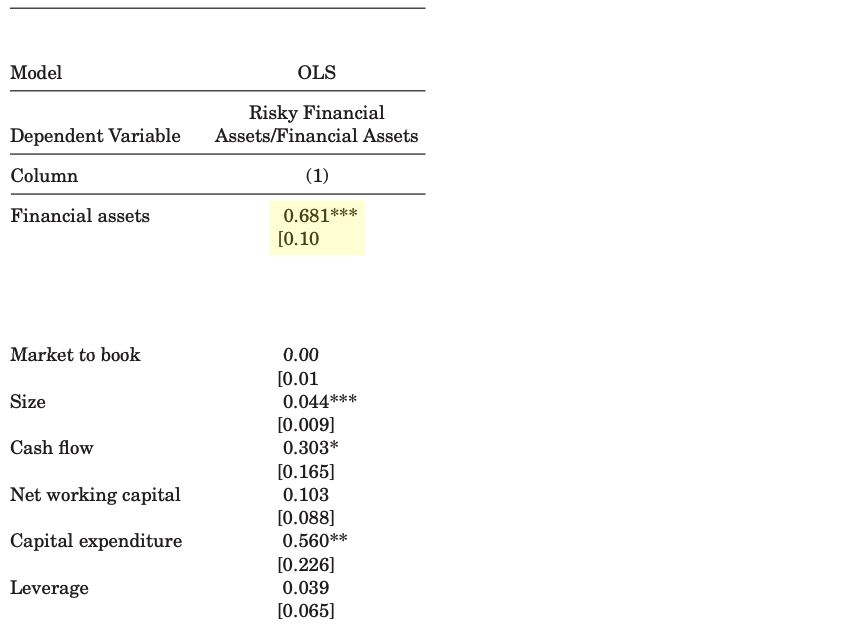
\includegraphics[scale=0.21]{regression_1_ols}

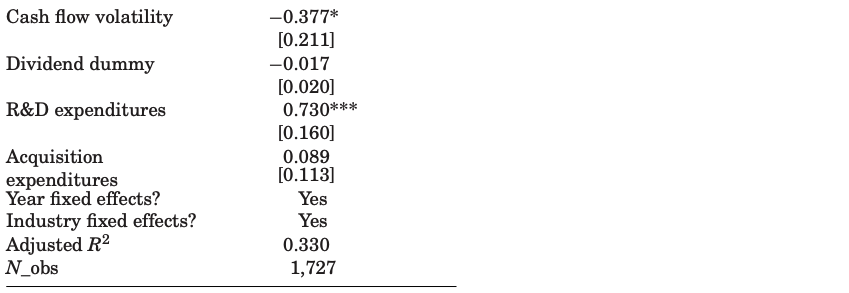
\includegraphics[scale=0.21]{regression_2_ols}

\end{frame}

\begin{frame}[label=endogeneity]
\frametitle{Endogeneity}

\begin{itemize}[<+->]
\item \textbf{Problem:} Firms likely jointly determine the size and composition of their financial portfolio.

\bigskip

$\implies$ A violation of the conditional mean independence assumption.

\bigskip

\item \textbf{Solution:} Use two-stage least squares to exploit the variation in the portfolio size due to unexpected cash flow shocks. \hyperlink{unexpected}{\beamerskipbutton{More}}
\end{itemize}

\end{frame}



\begin{frame}
\frametitle{2SLS Results}

\tiny

\begin{align*}
Financial \; assets_{i,t} &= \alpha_0 + \alpha_1 Unexpected \; cash \; flow_{i,t} + \beta' X_{i,t} + \sum_s year_s + \sum_j industry_j + \varepsilon_{i,t}^T\\
Risky \; financial \; assets_{i,t} &= \alpha_0 + \alpha_1 Financial \; assets_{i,t}^* + \beta' X_{i,t} + \sum_s year_s + \sum_j industry_j + \varepsilon_{i,t}^R
\end{align*}

\centering
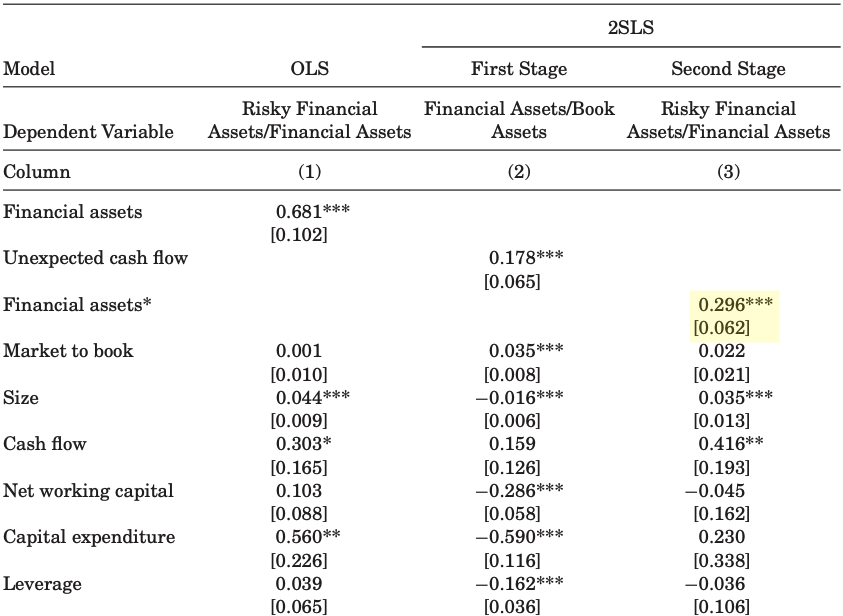
\includegraphics[scale=0.20]{regression_1_2sls}

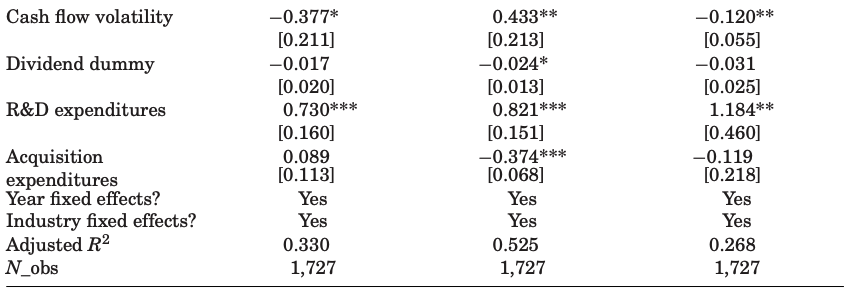
\includegraphics[scale=0.20]{regression_2_2sls}

\end{frame}



\begin{frame}
\frametitle{Other Findings}
\begin{itemize}[<+->]
\item Firms invest more in risky financial assets if they have

\begin{itemize}[<+->]
\item Worse corporate governance
\item An overconfident CEO
\end{itemize}

\bigskip

\item Industrial firms cannot generate a positive alpha through their risky financial asset holdings.

\bigskip

\item Develop a theory of industrial firms investing in risky and illiquid financial assets.

\begin{itemize}
\item Predictions that are consistent with their empirical analysis.
\end{itemize}

\end{itemize}

\end{frame}


\section{Concluding Thoughts}




\begin{frame}
\frametitle{Takeaways}
\begin{itemize}[<+->]
\item How we measure things is important. Make friends with accountants.
\bigskip
\item Have RAs.

\end{itemize}
\end{frame}




\section{Appendix}






\begin{frame}[label=APPL2007]
\frametitle{Apple 10-K (2007) Consolidated Balance Sheet}

\centering
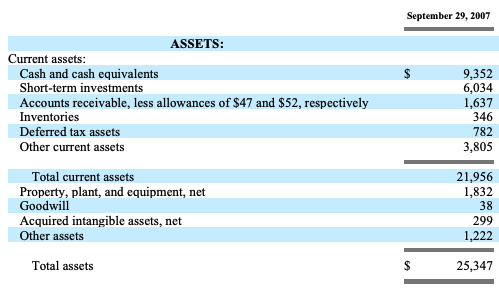
\includegraphics[scale=0.5]{AAPL_2007_bs}
\end{frame}







\begin{frame}
\frametitle{Apple 10-K (2007) Note 2 Financial Instruments}
 Cash, Cash Equivalents and Short-Term Investments.

\centering
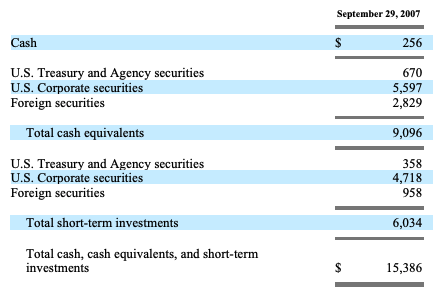
\includegraphics[scale=0.5]{AAPL_2007_note2}

\hyperlink{standardapproach}{\beamerskipbutton{Back}}
\end{frame}






\begin{frame}[label=APPL2011]
\frametitle{Apple 10-K (2011) Consolidated Balance Sheet}

\centering
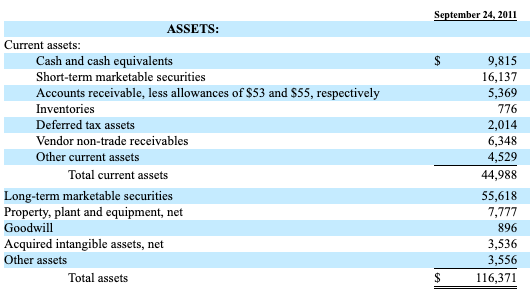
\includegraphics[scale=0.5]{AAPL_2011_bs}
\end{frame}






\begin{frame}
\frametitle{Apple 10-K (2011) Note 2 Financial Instruments}
 Cash, Cash Equivalents and Marketable Securities.

\centering
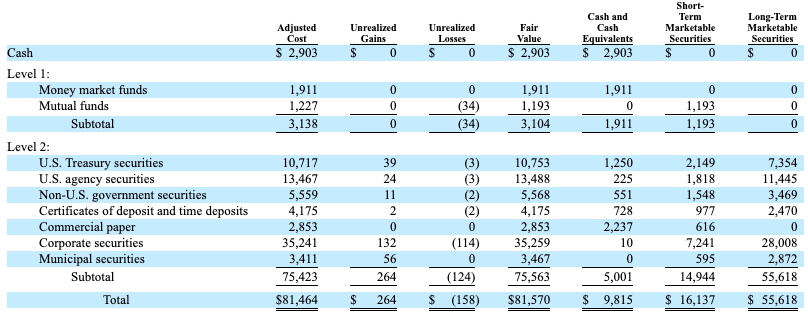
\includegraphics[scale=0.4]{AAPL_2011_note2}

\hyperlink{duchinapproach}{\beamerskipbutton{Back}}
\end{frame}







\begin{frame}[label=classify]
\frametitle{Classifying by Riskiness and Liquidity}
\begin{itemize}
\item Riskiness is based on the Fed's money supply definitions:
\begin{itemize}
\item $Safe$ is money-like (M4 and L). 
\item $Risky$ is nonmoney-like (the rest).
\end{itemize}
\item Liquidity is based on fair value levels:
\begin{itemize}
\item $Liquid$ is level 1 (market price available).
\item $Illiquid$ is level 2 and 3 (no market price available).
\end{itemize}
\bigskip
\item Example, equities are classified as risky and liquid.
\end{itemize}
\end{frame}







\begin{frame}
\frametitle{More on Riskiness}

\begin{columns}
\begin{column}{0.5\textwidth}

Safe financial assets

\begin{itemize}
\item Cash
\item Deposits
\item Commercial paper
\item Money market funds
\item U.S. Treasuries
\end{itemize}


\end{column}
\begin{column}{0.5\textwidth}

Risky financial assets

\begin{itemize}
\item Other government debt
\begin{itemize}
\item Munis
\item Agency
\item Foreign
\end{itemize}
\item Corporate
\item ABS and MBS
\item Equity
\item Other
\end{itemize}

\end{column}
\end{columns}

\bigskip

\hyperlink{duchinapproach}{\beamerskipbutton{Back}}


\end{frame}



\begin{frame}[label=unexpected]
\frametitle{Unexpected Cash Flows Shocks}
\begin{itemize}

\item Unexpected cash flow shocks ($e_{i,t}$) are estimated with the pooled cross-sectional time-series model below:

$$
\Delta CF_{i,t}
= \alpha + \beta_1 \Delta CF_{i,t-1} + \beta_2 \Delta CF_{i,t-2} + \beta_3 \Delta CF_{i,t-3} + e_{i,t}
$$

where $\Delta CF_{i,t} \equiv CF_{i,t} - CF_{i,t-1}$ and $CF_{i,t}$ is the cash flow for firm $i$ in year $t$.

\item Identifying assumptions:

\begin{itemize}

\item \textit{Inclusion restriction:} Unexpected cash flow shocks affect the size of the firm's financial portfolio.
\item \textit{Exclusion restriction:} Unexpected cash flow shocks do not affect the composition of the firm's financial portfolio.



\end{itemize}

\end{itemize}
\hyperlink{endogeneity}{\beamerskipbutton{Back}}
\end{frame}


\end{document}

